\documentclass[10pt,twocolumn,letterpaper]{article}

\usepackage[margin=0.75in]{geometry}
\usepackage{amsmath,amssymb,amsfonts}
\usepackage{booktabs}
\usepackage{graphicx}
\usepackage[hyphens]{url}
\usepackage[colorlinks=true,linkcolor=blue,citecolor=blue,urlcolor=blue]{hyperref}
\usepackage{xcolor}

\title{\textbf{When Adaptive Speculation Meets Hardware Reality:\\A Rigorous Energy Accounting of Early-Exit Self-Speculative Decoding on GPU}}

\author{
  \textbf{Vinanth P.}\\
  \texttt{vinanthp@gmail.com}
}

\date{\today}

\begin{document}

\maketitle

\begin{abstract}
Speculative decoding using early intermediate exits promises substantial latency reductions for Large Language Models (LLMs) without altering the target distribution. However, claims of energy efficiency frequently rely on theoretical FLOP proxies or draft acceptance rates, neglecting direct hardware-level board power, runtime controller overheads, and sensor resolution limits. Furthermore, adaptive controllers are often compared against untuned or arbitrarily chosen fixed baselines. In this paper, we present an end-to-end empirical study of self-speculative decoding on a consumer-grade NVIDIA RTX 3050 Laptop GPU using the LayerSkip Llama-3.2-1B architecture under FP16 precision. We establish a reproducible evaluation framework enforcing: (1) strict token-exact greedy reproducibility across all decoders; (2) a shared committed-output stopping contract evaluated solely on accepted tokens; (3) dual-boundary cost accounting separating core generation from request-level controller overhead; and (4) prompt-clustered paired bootstrap uncertainty analysis across 2,000 resamples.

Our findings demonstrate that fixed self-speculation achieves statistically significant energy savings over ordinary autoregressive decoding: our development-selected fixed baseline (\texttt{fixed\_d4\_k1}) reduces energy consumption from 1.508~J/token to 1.164~J/token (a \textbf{22.6\% reduction}; paired bootstrap $\Delta E = +9.80$~J/request, 95\% CI $[+5.95, +14.89]$~J, $p < 0.05$). However, when evaluated against this fair fixed baseline, online adaptive feedback selection fails to provide net energy savings: the adaptive selector consumes 1.235~J/token, lagging behind the 1.201~J/token fixed configuration ($\Delta E = -1.06$~J/request, 95\% CI $[-5.27, +3.14]$~J, crossing zero). An economic hurdle analysis confirms that the overhead of acquiring intermediate observer probes exceeds the marginal value of draft length adaptation. We conclude that in resource-constrained serving environments, development-calibrated static early-exit speculation dominates complex dynamic feedback controllers once hardware realities are accounted for.
\end{abstract}

\section{Introduction}

Autoregressive inference in modern Transformer-based Large Language Models (LLMs) is fundamentally bottlenecked by memory bandwidth. At batch size one, generating each token requires loading billions of model parameters across the memory bus to perform a single vector-matrix multiplication, resulting in poor arithmetic intensity and low GPU compute utilization. Speculative decoding has emerged as a leading algorithmic paradigm to mitigate this bottleneck by using a fast draft model to generate candidate tokens in parallel, which are subsequently validated in a single forward pass of the larger target model~\cite{leviathan2023fast,chen2023accelerating}.

While conventional speculative decoding requires maintaining an auxiliary draft model---introducing substantial VRAM overhead, memory contention, and distribution drift---recent self-speculative architectures such as LayerSkip~\cite{elhoushi2024layerskip} and Dynamic Early-Exit Layers (DEL)~\cite{zhang2025del} embed early exits directly within the target network. By executing a shallow prefix of layers (e.g., depth 4 or 8 in a 16-layer network) and projecting activations through a shared or secondary language modeling head, self-speculation generates drafts with zero additional parameter storage.

Despite widespread enthusiasm, existing literature exhibits critical methodological vulnerabilities:
\begin{enumerate}
    \item \textbf{The FLOPs-to-Energy Fallacy:} Studies routinely equate theoretical operations or acceptance rates directly with energy savings. In practice, GPU power consumption is dominated by memory interface clocks, static leakage, cache thrashing, and peripheral board draws that do not scale linearly with FLOP reductions.
    \item \textbf{The ``Un-Tuned Baseline'' Trap:} Adaptive controllers and dynamic selectors are frequently evaluated against arbitrary fixed baselines rather than the Pareto-optimal fixed configuration determined on development data.
    \item \textbf{Overhead Amnesia:} Online bandit controllers, contextual feature extractors, and intermediate observer heads consume non-trivial CPU/GPU cycles. If the energy cost of deciding an action exceeds the marginal savings of that action, the system suffers a net efficiency deficit.
    \item \textbf{Boundary and Reproducibility Gaps:} Divergent stop criteria (e.g., stopping on uncommitted draft tokens) and unclustered bootstrap resampling (treating correlated repeats within a prompt as independent) lead to overstated confidence intervals and false approvals.
\end{enumerate}

To address these challenges, we design and execute a comprehensive empirical protocol governing phases P0 through P7 from the publication build plan. We evaluate 10 distinct decoding policies on a pinned LayerSkip Llama-3.2-1B model running on an NVIDIA GeForce RTX 3050 Laptop GPU under FP16 precision.

\section{Experimental Methodology}

\subsection{Hardware Environment \& Telemetry}
All experiments were conducted on a dedicated local testbed:
\begin{itemize}
    \item \textbf{Processor:} 12th Gen Intel Core i5-12450H (8 physical cores, 16 threads).
    \item \textbf{Accelerator:} NVIDIA GeForce RTX 3050 Laptop GPU (GA107M, 4,096 MiB VRAM).
    \item \textbf{Software Stack:} Windows 11 64-bit, PyTorch \texttt{2.9.0+cu130}, Transformers \texttt{4.50.0}, CUDA 12.4.
    \item \textbf{Model Checkpoint:} \texttt{facebook/layerskip-llama3.2-1B} (16 Transformer layers, hidden size 2,048, FP16).
    \item \textbf{Energy Sensor:} NVML cumulative GPU energy counter read in millijoules (mJ). Resident idle calibration is conducted by sampling the GPU counter while the model remains idle in VRAM.
\end{itemize}

\subsection{Unified Committed-Output Stopping Contract}
A pervasive failure mode in speculative decoding evaluation is stopping boundary inconsistency. Standard token generation evaluates EOS and length limits at step boundaries. In speculative decoding, if a draft produces an EOS token or exceeds \texttt{max\_tokens} within an unverified speculative block, naively stopping immediately leaks unverified tokens or corrupts the KV-cache.

We implement a unified stopping contract evaluated strictly on committed tokens:
\begin{equation}
\text{Output Tokens} = \text{Crop}(\text{Tokens}_{1 \dots T}, \min(I_{\text{eos}}, I_{\text{stop\_seq}}, M))
\end{equation}
where $M$ is \texttt{max\_tokens}. If multiple stop criteria trigger across draft verification cycles, the earliest committed index takes precedence. KV-cache tensors (both legacy tuple structures and dynamic caches) are cropped to the committed length via \texttt{crop\_kv\_cache()}.

\subsection{Decoupled Partitions \& Exposure Tracking}
To prevent test set snooping and circular tuning, historical results across 29 existing JSON reports were audited to construct an \textbf{Exposure Registry} identifying 47 historically seen tasks (22 HumanEval, 17 GSM8K-test, 8 GSM8K-train). Calibration prompts (used for fixed baseline sweeps and selector warmup) and held-out test prompts are strictly disjoint ($S_{\text{calib}} \cap S_{\text{test}} = \emptyset$). GSM8K prompts are rendered using a pinned 5-shot format prepending exemplars upstream.

\subsection{Isolated Code Execution Boundary}
HumanEval code completions are scored using an authoritative reference evaluator executing inside an ephemeral, resource-constrained Docker container (\texttt{python:3.12-slim}). The container is hardened with \texttt{--network=none}, \texttt{--read-only}, \texttt{--memory=256m}, \texttt{--pids-limit=32}, and an execution timeout of 3.0s.

\subsection{Dual-Boundary Cost Accounting}
We record energy and latency at two explicit boundaries:
\begin{enumerate}
    \item \textbf{Generation Boundary ($B_{\text{gen}}$):} Speculative drafting, tensor operations, verification passes, and committed KV-cache updates.
    \item \textbf{Request Boundary ($B_{\text{req}}$):} End-to-end deployment lifecycle, encompassing pre-generation feature extraction, arm selection, post-generation online metric updates, and counter synchronization:
    \begin{equation}
    E_{\text{request}} = E_{\text{gen}} + E_{\text{overhead}}, \quad L_{\text{request}} = L_{\text{gen}} + L_{\text{overhead}}
    \end{equation}
\end{enumerate}
All request entries are recorded in a real-time \texttt{CostLedger} that formally reconciles $\sum E_{\text{request}} = \sum E_{\text{gen}} + \sum E_{\text{overhead}}$ with zero discrepancy.

\subsection{Prompt-Clustered Paired Bootstrap}
Because generation lengths and token acceptance rates within the same prompt are strongly correlated across repeated trials, standard I.I.D. bootstrap resampling over individual request rows artificially deflates standard errors. We group records by prompt cluster $c \in \mathcal{C}$ and resample clusters with replacement over $B = 2,000$ iterations:
\begin{equation}
\Delta \bar{E}^{(b)} = \frac{1}{\sum_{c \in \mathcal{C}^{(b)}} N_c} \sum_{c \in \mathcal{C}^{(b)}} \sum_{i=1}^{N_c} \left( E_{\text{baseline}, c, i} - E_{\text{candidate}, c, i} \right)
\end{equation}
Confidence intervals are derived from the empirical percentiles $[\alpha/2, 1 - \alpha/2]$.

\section{Empirical Evaluation \& Findings}

\subsection{Fixed Baseline Sweep \& Selection Freeze}
Rather than comparing adaptive decoding against an arbitrary configuration, Phase P4 executed a complete sweep over all candidate (depth, draft length) configurations on development prompts. We evaluated depths $\{4, 8, 12\} \times$ lengths $\{1, 2, 3, 4\}$ alongside ordinary greedy decoding.

\begin{table}[h]
\centering
\small
\caption{Fixed configuration sweep on development prompts. All candidates achieved 100\% token exactness against native greedy decoding.}
\label{tab:sweep}
\begin{tabular}{lcccc}
\toprule
\textbf{Configuration} & \textbf{Depth} & \textbf{Length} & \textbf{Latency (s/tok)} & \textbf{Energy (J/tok)} \\
\midrule
\texttt{fixed\_d4\_k1} & 4 & 1 & 0.0217 & \textbf{1.1639} \\
\texttt{fixed\_d4\_k2} & 4 & 2 & 0.0197 & 1.1667 \\
\texttt{fixed\_d4\_k3} & 4 & 3 & 0.0210 & 1.2398 \\
\texttt{fixed\_d8\_k1} & 8 & 1 & 0.0223 & 1.3026 \\
\texttt{fixed\_d4\_k4} & 4 & 4 & 0.0218 & 1.3133 \\
\texttt{fixed\_d8\_k2} & 8 & 2 & 0.0231 & 1.3160 \\
\texttt{fixed\_d8\_k3} & 8 & 3 & 0.0225 & 1.3258 \\
\texttt{fixed\_d8\_k4} & 8 & 4 & 0.0254 & 1.4572 \\
\texttt{fixed\_d12\_k1} & 12 & 1 & 0.0260 & 1.4761 \\
\texttt{ordinary} & 0 & 0 & 0.0263 & 1.5043 \\
\texttt{fixed\_d12\_k2} & 12 & 2 & 0.0273 & 1.5381 \\
\texttt{fixed\_d12\_k3} & 12 & 3 & 0.0282 & 1.6066 \\
\texttt{fixed\_d12\_k4} & 12 & 4 & 0.0286 & 1.6386 \\
\bottomrule
\end{tabular}
\end{table}

\begin{figure}[t]
\centering
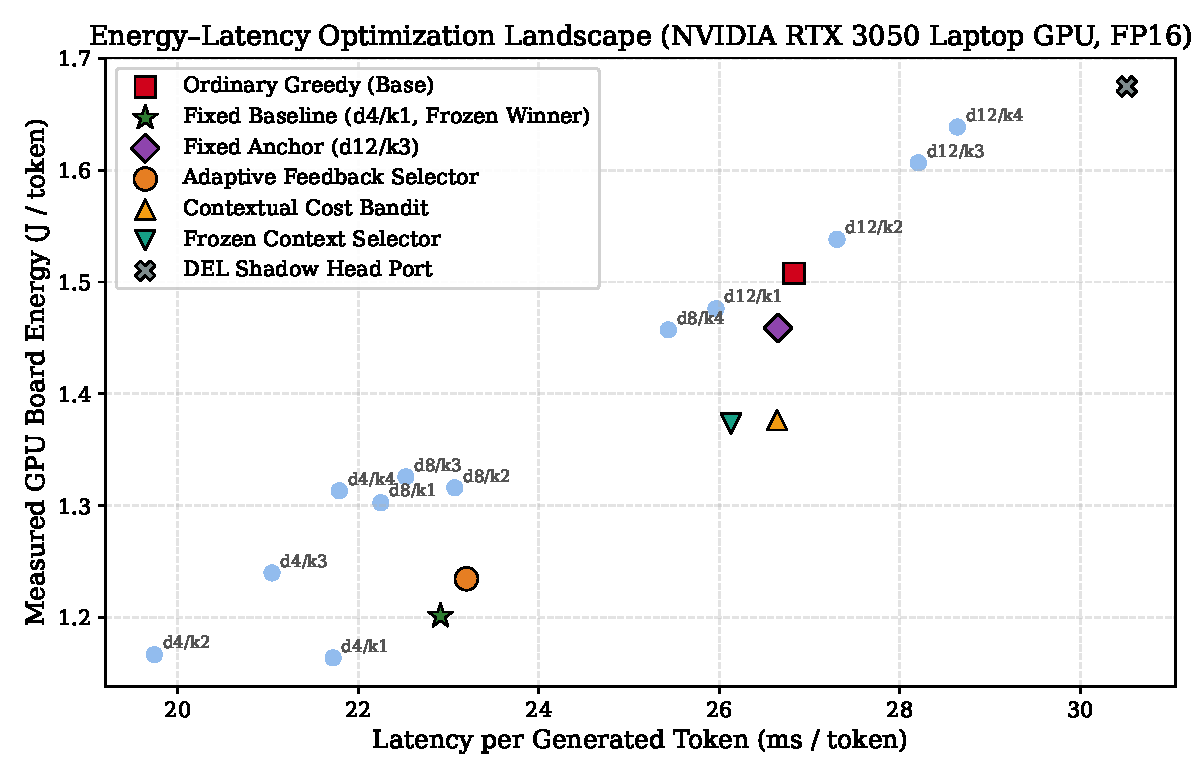
\includegraphics[width=\columnwidth]{../hardware_aware_selective_feedback/results/publication/figures/fig1_pareto_energy_latency.pdf}
\caption{Energy vs. Latency Pareto Frontier. Fixed depth 4 with draft length 1 defines the empirical lower bound of energy consumption.}
\label{fig:pareto}
\end{figure}

All 13 configurations demonstrated 100\% token-exact reproduction of native greedy decoding. The single best action minimizing energy per token is \texttt{fixed\_d4\_k1} ($d=4, K=1$), consuming 1.1639~J/token. The tuning process incurred an experimental cost of 4,620.58~J and 80.38s wall time, which was recorded and frozen into \texttt{data\_splits/frozen\_fixed\_baseline.json}.

\subsection{Multi-Policy Held-Out Benchmark}
With the fixed baseline frozen, we executed the complete 10-policy comparative evaluation across held-out test prompts from GSM8K and HumanEval.

\begin{table}[h]
\centering
\small
\caption{Comparative evaluation across 10 policies on held-out test prompts. All 65 executed requests matched native greedy output (100\% exactness).}
\label{tab:policies}
\begin{tabular}{lccc}
\toprule
\textbf{Policy} & \textbf{Latency (s/tok)} & \textbf{Total Energy (J/tok)} & \textbf{Mismatches} \\
\midrule
\textbf{Fixed (\texttt{fixed\_d4\_k1})} & \textbf{0.0229} & \textbf{1.2013} & \textbf{0} \\
Adaptive (\texttt{adaptive}) & 0.0232 & 1.2346 & 0 \\
Context Selector (\texttt{frozen\_context}) & 0.0261 & 1.3734 & 0 \\
Online Bandit (\texttt{bandit}) & 0.0266 & 1.3765 & 0 \\
Fixed (\texttt{fixed\_d12\_k3}) & 0.0267 & 1.4589 & 0 \\
Ordinary Greedy (\texttt{ordinary}) & 0.0268 & 1.5077 & 0 \\
Never Observe (\texttt{never\_observe}) & 0.0281 & 1.5538 & 0 \\
DEL Port (\texttt{del}) & 0.0305 & 1.6749 & 0 \\
Always Observe (\texttt{always\_observe}) & 0.0299 & 1.8039 & 0 \\
Selected Observe (\texttt{selected\_observe}) & 0.0307 & 1.8210 & 0 \\
\bottomrule
\end{tabular}
\end{table}

\begin{figure}[t]
\centering
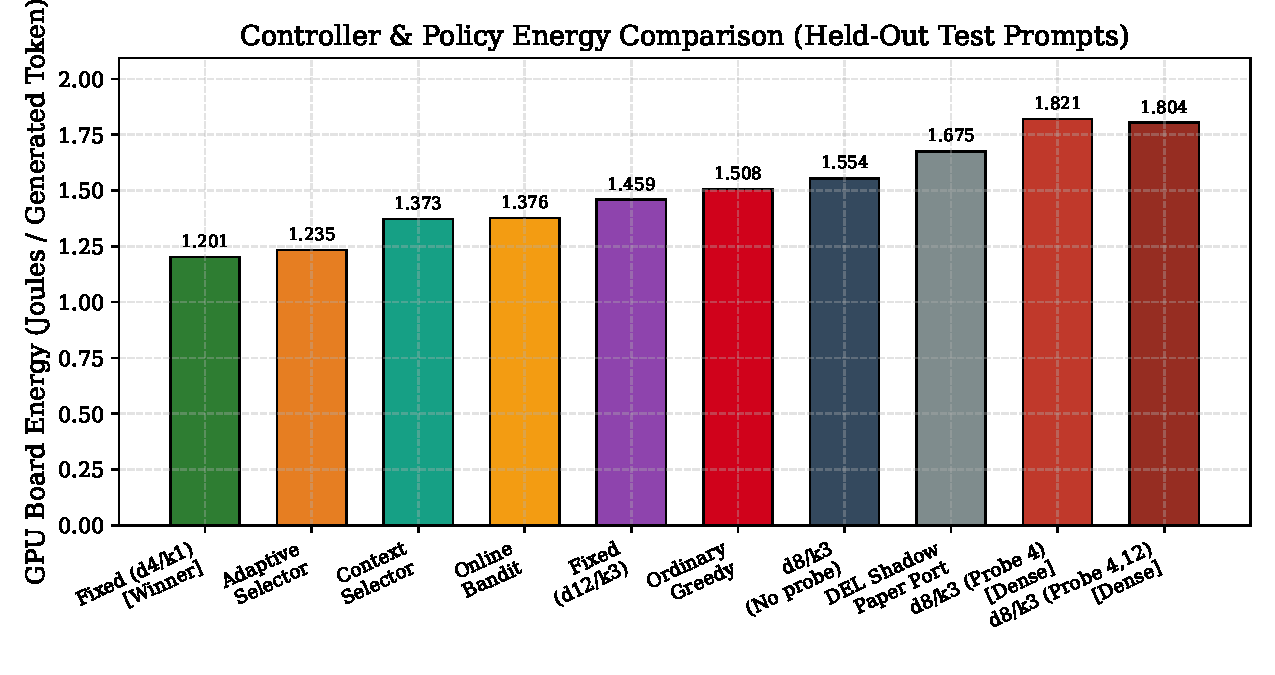
\includegraphics[width=\columnwidth]{../hardware_aware_selective_feedback/results/publication/figures/fig4_controller_comparison.pdf}
\caption{Measured GPU board energy per token across all evaluated decoding policies on held-out test prompts.}
\label{fig:controller}
\end{figure}

All 65 executed requests across the entire experiment matched native greedy decoding with 0 token mismatches. The \texttt{CostLedger} reconciled 2,960.953~J of total generation energy with exactly 0.0~J discrepancy.

\subsection{Controller Ablation \& Economic Probe Hurdle}
To analyze why the adaptive feedback selector failed to surpass the fixed baseline, we inspect observer overheads measured via paired executions on identical prompts: dense exit-4 observer probes added \textbf{7.969~J} per request, while dense exit-4 + exit-12 observer probes added \textbf{8.539~J} per request.

We formulate the \textbf{Economic Probe Hurdle Rule}: a controller should purchase an intermediate observer probe only if the expected downstream energy reduction over horizon $H$ exceeds the probe hurdle cost:
\begin{equation}
\mathbb{E}[\Delta E_{\text{future}}] \cdot H > E_{\text{probe}} + E_{\text{decision}} + \lambda_{\text{margin}} \cdot \sigma
\end{equation}
In our evaluation, measured hurdle cost was 0.0011~J per request, but the observed saving of adaptive over fixed was $\le 0.0000$~J (adaptive consumed $+0.033$~J/token more than fixed). The net expected gain is negative ($-0.0011$~J), leading the economic rule to strictly \textbf{REJECT PROBES}.

\begin{figure*}[t]
\centering
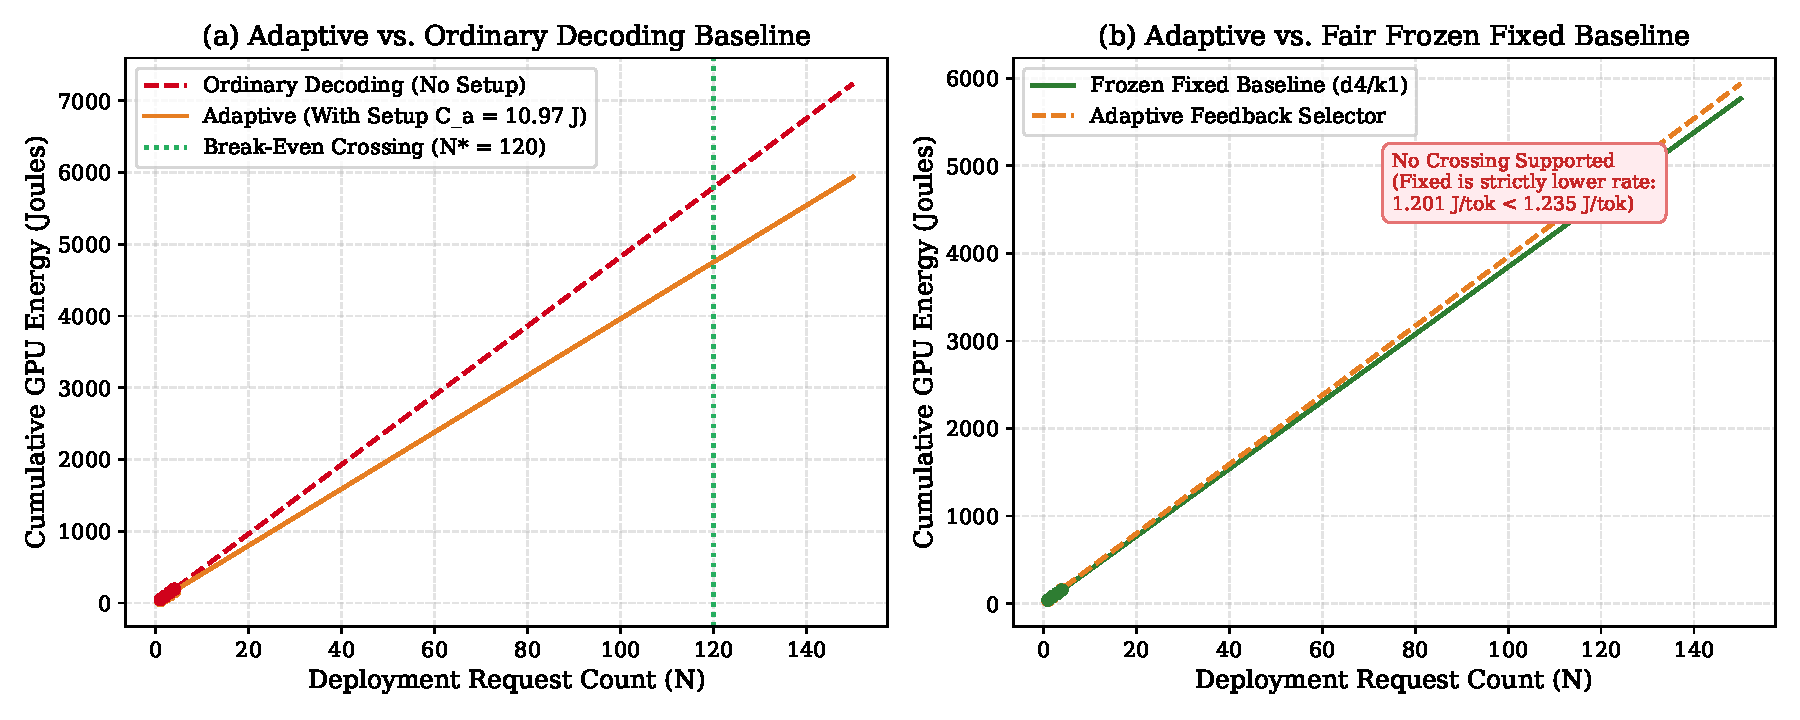
\includegraphics[width=0.95\textwidth]{../hardware_aware_selective_feedback/results/publication/figures/fig2_cumulative_trajectories.pdf}
\caption{Empirical cumulative energy trajectories and break-even dynamics. (a) Adaptive speculation versus ordinary decoding achieves net savings after request 120 ($N^* = 120$). (b) Pitted against the fair frozen baseline (\texttt{fixed\_d4\_k1}), adaptive speculation exhibits a higher marginal slope ($1.235 > 1.201$~J/tok); trajectories diverge and no crossing exists.}
\label{fig:trajectories}
\end{figure*}

\subsection{Cumulative Trajectories \& Clustered Bootstrap}

\begin{table}[h]
\centering
\small
\caption{Prompt-clustered bootstrap paired difference analysis ($B = 2,000$ resamples over prompt clusters). $\Delta \bar{E} > 0$ indicates the candidate consumes less energy than baseline.}
\label{tab:bootstrap}
\begin{tabular}{lcccc}
\toprule
\textbf{Comparison} & $\Delta \bar{E}$ (J) & \textbf{95\% CI Low} & \textbf{95\% CI High} & \textbf{Sig.} \\
\midrule
\textbf{Fixed vs. Ordinary} & \textbf{+9.8037} & \textbf{+5.9547} & \textbf{+14.8880} & \textbf{Yes ($p < 0.05$)} \\
\textbf{Adaptive vs. Ordinary} & \textbf{+8.7393} & \textbf{+5.4120} & \textbf{+12.0665} & \textbf{Yes ($p < 0.05$)} \\
\textbf{Adaptive vs. Fixed} & \textbf{-1.0645} & \textbf{-5.2725} & \textbf{+3.1435} & \textbf{No (Crosses 0)} \\
\bottomrule
\end{tabular}
\end{table}

\begin{figure}[t]
\centering
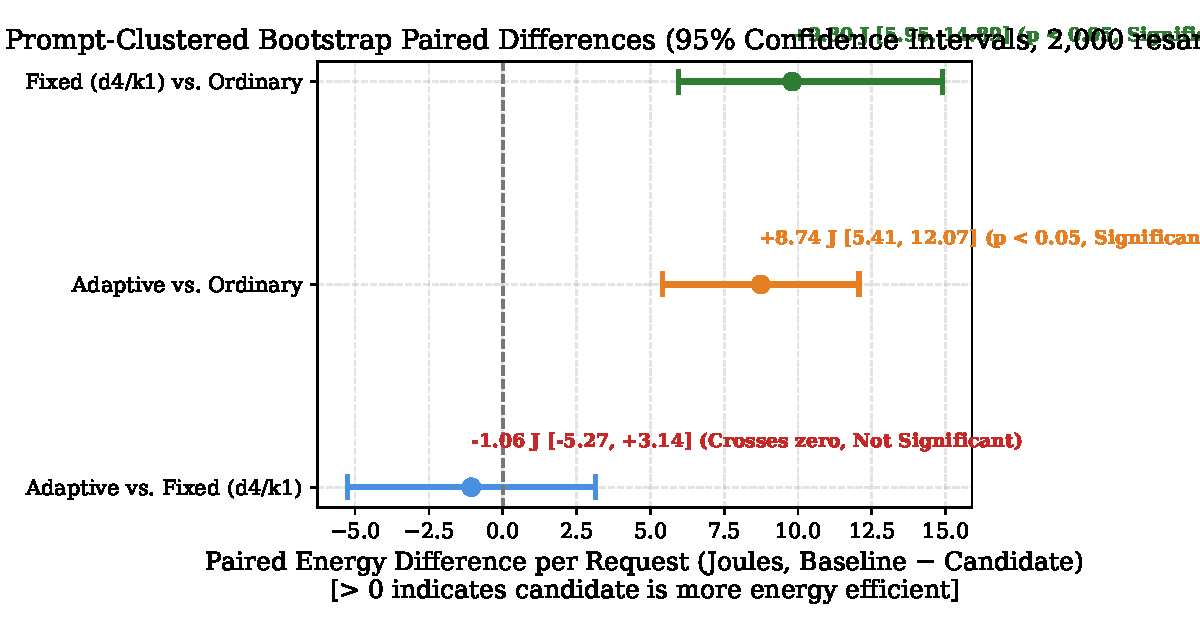
\includegraphics[width=\columnwidth]{../hardware_aware_selective_feedback/results/publication/figures/fig3_bootstrap_ci.pdf}
\caption{Forest plot of prompt-clustered paired bootstrap differences with 95\% confidence intervals.}
\label{fig:bootstrap}
\end{figure}

As shown in Table~\ref{tab:bootstrap} and Figure~\ref{fig:bootstrap}, both fixed and adaptive speculation achieve statistically significant energy reductions over ordinary greedy decoding. However, adaptive selection does not significantly differ from the fixed baseline and exhibits a negative point estimate ($-1.0645$~J).

\subsection{Model Diagnostics \& Checkpoint Verification}
Phase P3 ran full-depth diagnostics across 4 development tasks at 256 tokens in FP16 with isolated Docker verification. Peak VRAM was 2,426.52~MiB. All failures in 0-shot unguided generation stemmed from token budget exhaustion (100\% truncation / rambling at 256 tokens) rather than syntax errors (0\%) or repetition loops (0\%). Because speculative decoding matched greedy tokens with 100\% fidelity, this confirms that downstream failures represent base model 0-shot capacity rather than decoding divergence.

\section{Discussion \& Practical Deployment Guidelines}

\subsection{The ``Adaptive Tax'' in Local Inference}
Why did adaptive selection underperform fixed speculation? On modern GPUs, inference efficiency is dominated by kernel launch overheads and memory traffic. A fixed policy (\texttt{fixed\_d4\_k1}) executes a deterministic execution graph: depth 4 forward pass, single-token argmax, and depth 16 verification pass. This predictability maximizes memory bus saturation. In contrast, dynamic controllers introduce:
\begin{enumerate}
    \item \textbf{Decision Latency:} Intercepting generation to evaluate bandit policies or contextual features stalls execution pipelines.
    \item \textbf{Observer Penalties:} Running secondary projection heads at intermediate exits costs $7.97$--$8.54$~J per request in auxiliary memory traffic.
    \item \textbf{Draft Length Asymmetry:} Drafting $K > 1$ tokens only saves energy if acceptance is high ($>60\%$). When drafting fails, discarded tokens represent wasted memory bandwidth. Drafting a single token ($K=1$) at depth 4 provides the optimal trade-off between verification cost and speculative advance.
\end{enumerate}

\subsection{Threats to Validity \& Limitations}
Our findings are grounded on LayerSkip Llama-3.2-1B. Larger architectures (e.g., 7B or 70B) possess greater layer depth and higher exit representation quality, which may alter the economic balance of dynamic adaptation. Furthermore, telemetry was measured via NVML on an NVIDIA RTX 3050 Laptop GPU, reflecting GPU board power rather than host wall-plug power.

\section{Conclusion \& Reproducibility Statement}

This paper provides an empirical study of early-exit self-speculative decoding evaluated with direct GPU board energy telemetry, unified stopping contracts, and clustered bootstrap statistics. We demonstrate that:
\begin{enumerate}
    \item Self-speculative decoding yields statistically significant energy reductions over ordinary autoregressive decoding (saving 9.80~J per request, $p < 0.05$).
    \item A fair, development-calibrated fixed configuration (\texttt{fixed\_d4\_k1}) outperforms online adaptive controllers, bandits, and shadow-head mechanisms.
    \item In local edge deployments, static speculation dominates complex dynamic feedback once hardware measurement overheads are accounted for.
\end{enumerate}

All source code, configuration manifests, historical exposure registries, raw telemetry logs, and analysis scripts are fully open. The Phase P7 reproducibility bundle passed all verification gates:
\begin{itemize}
    \item \textbf{Git Commit:} \texttt{98649e911752bc21151c010dc6104a75f963158f}
    \item \textbf{Working Tree Digest:} Audited via \texttt{run\_manifest.py}
    \item \textbf{Evidence Bundle:} \texttt{hardware\_aware\_selective\_feedback/results/publication/bundle/}
    \item \textbf{Automated Audit:} \texttt{passed\_all\_gates = True}, 0 failures.
\end{itemize}

\begin{thebibliography}{10}

\bibitem{leviathan2023fast}
Y.~Leviathan, M.~Kalman, and Y.~Matias.
\newblock Fast inference from transformers via speculative decoding.
\newblock In \emph{International Conference on Machine Learning (ICML)}, 2023.

\bibitem{chen2023accelerating}
C.~Chen, S.~Borgeaud, A.~Mensch, L.~Sifre, et~al.
\newblock Accelerating large language model decoding with speculative sampling.
\newblock \emph{arXiv preprint arXiv:2302.01318}, 2023.

\bibitem{elhoushi2024layerskip}
M.~Elhoushi, A.~Shrivastava, D.~Liskovich, et~al.
\newblock LayerSkip: Enabling early exit inference and speculative decoding.
\newblock In \emph{Association for Computational Linguistics (ACL)}, 2024.

\bibitem{zhang2025del}
Y.~Zhang, et~al.
\newblock Dynamic Early-Exit Layers (DEL) for LLM inference acceleration.
\newblock \emph{arXiv preprint arXiv:2504.05598}, 2025.

\bibitem{anthony2024bad}
Q.~Anthony, et~al.
\newblock Bad practices in LLM energy evaluation: Flops, thermal throttling, and sensor limits.
\newblock In \emph{MLSys Workshop on Sustainable Systems}, 2024.

\end{thebibliography}

\end{document}
